\let\negmedspace\undefined
\let\negthickspace\undefined
\documentclass[journal]{IEEEtran}
\usepackage[a5paper, margin=10mm, onecolumn]{geometry}
%\usepackage{lmodern} % Ensure lmodern is loaded for pdflatex
\usepackage{tfrupee} % Include tfrupee package

\setlength{\headheight}{1cm} % Set the height of the header box
\setlength{\headsep}{0mm}     % Set the distance between the header box and the top of the text

\usepackage{gvv-book}
\usepackage{gvv}
\usepackage{cite}
\usepackage{amsmath,amssymb,amsfonts,amsthm}
\usepackage{algorithmic}
\usepackage{graphicx}
\usepackage{textcomp}
\usepackage{xcolor}
\usepackage{txfonts}
\usepackage{listings}
\usepackage{enumitem}
\usepackage{mathtools}
\usepackage{gensymb}
\usepackage{comment}
\usepackage[breaklinks=true]{hyperref}
\usepackage{tkz-euclide} 
\usepackage{listings}
% \usepackage{gvv}                                        
\def\inputGnumericTable{}                                 
\usepackage[latin1]{inputenc}                                
\usepackage{color}                                            
\usepackage{array}                                            
\usepackage{longtable}                                       
\usepackage{calc}                                             
\usepackage{multirow}                                         
\usepackage{hhline}                                           
\usepackage{ifthen}                                           
\usepackage{lscape}
\begin{document}

\bibliographystyle{IEEEtran}
\vspace{3cm}

\title{
1-Vector Arithmetic \\
\large EE1030:Matrix Theory
}
\author{Gajjarapu Satyanarayana\\AI24BTECH11009
}
% \maketitle
% \newpage
% \bigskip
{\let\newpage\relax\maketitle}

\renewcommand{\thefigure}{\theenumi}
\renewcommand{\thetable}{\theenumi}



\numberwithin{equation}{enumi}
\numberwithin{figure}{enumi}
\renewcommand{\thetable}{\theenumi}


\textbf{Question}:1.11.2\\
Unit vector along PQ, where coordinates of $\vec{P}$ and $\vec{Q}$ respectively are (2, 1, -1) and (4, 4, -7), is \hfill(12, 2023)
\\
\textbf{Solution:}
\renewcommand{\tablename}{Table 1.11.2.1}
\begin{table}[h!]
  \centering
  \begin{tabular}[12pt]{ |c| c|}
    \hline
    \textbf{Variables} & \textbf{Description}\\ 
    \hline
    $\textbf{V}_1, \vec{u}_1, f_1$ & Parameters of the parabola $y^2 = 4x$ \\
    \hline
     $\textbf{V}_2, \vec{u}_2, f_2$ & Parameters of the circle $4x^2 + 4xy^2 = 9$ \\
    \hline
    $\vec{x}^\intercal\brak{\textbf{V}_1 + \mu\textbf{V}_2}\vec{x} + 2\brak{\vec{u}_1 + \mu\vec{u}_2}^\intercal\vec{x} + \brak{f_1 + \mu f_2}$ & Intersection of two conics \\
    \hline
    \end{tabular}


  \caption{Vertex and its coordinates}
\end{table}
\\
The vector along PQ is $\vec{Q}$ - $\vec{P}$
    \begin{align}
    \vec{Q} - \vec{P} & = \myvec{4 \\ 4 \\ -7} - \myvec{2 \\ 1 \\ -1} \\
    \vec{Q} - \vec{P} & = \myvec{2 \\ 3 \\ -6} \\
    \brak{\vec{Q} - \vec{P}}^\intercal & = \myvec{2 & 3 & -6}
 \end{align}
The magnitude of the vector along PQ is
\begin{align}
\norm{\vec{Q} - \vec{P}} & = \sqrt{\brak{\vec{Q} - \vec{P}}^\intercal\brak{\vec{Q} - \vec{P}}} \\
   \norm{\vec{Q} - \vec{P}} & = \sqrt{\myvec{2 & 3 & -6} \myvec{2 \\ 3 \\ -6}} \\
   \norm{\vec{Q} - \vec{P}} & = \sqrt{\brak{2}^2 + \brak{3}^2 + \brak{-6}^2} \\
   \norm{\vec{Q} - \vec{P}} & = \sqrt{49} \\
   \norm{\vec{Q} - \vec{P}} & = 7 
\end{align}
The unit vector along PQ is 
\begin{align}
    \frac{\vec{Q} - \vec{P}}{\norm{\vec{Q} - \vec{P}}} & = \frac{\myvec{2 \\ 3 \\-6}}{7} \\
    \frac{\vec{Q} - \vec{P}}{\norm{\vec{Q} - \vec{P}}} & = \frac{1}{7}\myvec{2 \\ 3 \\ -6}
\end{align}
\begin{figure}[h!]
   \centering
   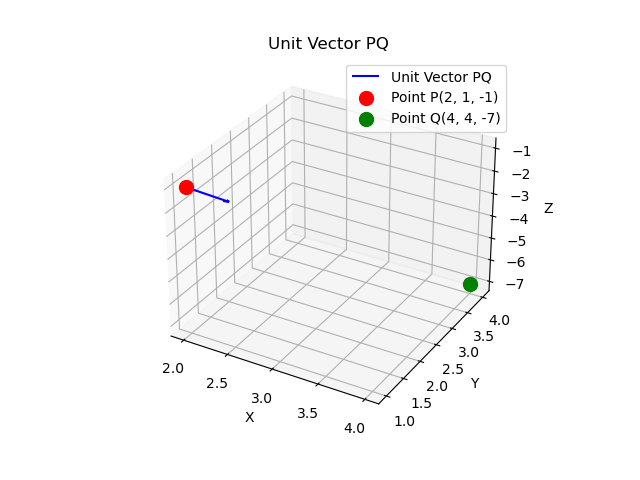
\includegraphics[width=0.7\linewidth]{figs/unit.png}
	\caption{Unit Vector PQ}
   \end{figure}
   \end{document}

